\documentclass{beamer}
\usepackage[utf8]{inputenc}

\usetheme{Madrid}
\usecolortheme{default}
\usepackage{amsmath,amssymb,amsfonts,amsthm}
\usepackage{txfonts}
\usepackage{tkz-euclide}
\usepackage{listings}
\usepackage{adjustbox}
\usepackage[T1]{fontenc}
\usepackage{array}
\usepackage{tabularx}
\usepackage{gvv}
\usepackage{lmodern}
\usepackage{circuitikz}
\usepackage{tikz}
\usepackage{graphicx}

\setbeamertemplate{page number in head/foot}[totalframenumber]

\usepackage{tcolorbox}
\tcbuselibrary{minted,breakable,xparse,skins}



\definecolor{bg}{gray}{0.95}
\DeclareTCBListing{mintedbox}{O{}m!O{}}{%
  breakable=true,
  listing engine=minted,
  listing only,
  minted language=#2,
  minted style=default,
  minted options={%
    linenos,
    gobble=0,
    breaklines=true,
    breakafter=,,
    fontsize=\small,
    numbersep=8pt,
    #1},
  boxsep=0pt,
  left skip=0pt,
  right skip=0pt,
  left=25pt,
  right=0pt,
  top=3pt,
  bottom=3pt,
  arc=5pt,
  leftrule=0pt,
  rightrule=0pt,
  bottomrule=2pt,
  toprule=2pt,
  colback=bg,
  colframe=orange!70,
  enhanced,
  overlay={%
    \begin{tcbclipinterior}
    \fill[orange!20!white] (frame.south west) rectangle ([xshift=20pt]frame.north west);
    \end{tcbclipinterior}},
  #3,
}
\lstset{
    language=C,
    basicstyle=\ttfamily\small,
    keywordstyle=\color{blue},
    stringstyle=\color{orange},
    commentstyle=\color{green!60!black},
    numbers=left,
    numberstyle=\tiny\color{gray},
    breaklines=true,
    showstringspaces=false,
}
%------------------------------------------------------------
%This block of code defines the information to appear in the
%Title page
\title %optional
{ 4.12.23}

%\subtitle{A short story}

\author % (optional)
{Hemanth Reddy-AI25BTECH11018}



\begin{document}


\frame{\titlepage}
\begin{frame}{Question}
A point moves so that square of its distance from the point (3, -2) is numerically
equal to its distance from the line 5x - 12y = 3. The equation of its locus is
\end{frame}



\begin{frame}{Theoretical Solution}
\textbf{Solution:}\\

\begin{align}
   \text{ Let the position vector of point }  \vec{P} \text{ is }
   = \myvec{ x \\ y} \\
  \text{  Let }\vec{a} = \myvec{ 3 \\ -2} 
\end{align}
Square of distance of point $\vec{P}$ from $\vec{a}$ is $\norm{\vec{P} -\vec{a} }^{2}$ = $(\vec{P} -\vec{a})^{T} (\vec{P} -\vec{a})$\\

\begin{align}
    (\vec{P} -\vec{a}) = \myvec{ x-3 \\ y+2} 
\end{align}

\begin{align}
    (\vec{P} -\vec{a})^{T}(\vec{P} -\vec{a})= \myvec{ x-3 & y+2}\myvec{ x-3 \\ y+2} = (x-3)^{2}+(y+2)^{2}
\end{align}





\end{frame}
\begin{frame}{Theoretical Solution}
\begin{align}
     \text{Let} \quad \vec{n} = \myvec{ 5 \\-12}  \\
     |\textbf{n}| = \sqrt{\textbf{n}^T \textbf{n}} = \sqrt{\myvec{ 5 & -12} \myvec{ 5 \\-12}} = \sqrt{25+144} = 13 
\end{align}

\begin{align}
    d = \frac{|\textbf{P}^T \textbf{n} - 3|}{|\textbf{n}|} = \frac{|5x - 12y - 3|}{13}
\end{align}

\begin{align}
   (x-3)^{2}+(y+2)^{2}= d = \frac{|5x - 12y - 3|}{13}
\end{align}



\end{frame}

\begin{frame}{Theoretical Solution}
\begin{align}
     (x-3)^{2}+(y+2)^{2}= \frac{(5x - 12y - 3)}{13}\\
13x^2 + 13y^2 - 83x + 64y + 172 = 0
\end{align}


The locus of the point is a circle.

\end{frame}

\begin{frame}[fragile]
    \frametitle{C Code }
    \begin{lstlisting}

#include <stdio.h>
#include <math.h>

int main() {
    // Fixed point coordinates
    double a_x = 3.0;
    double a_y = -2.0;

    // Line coefficients (Ax + By + C = 0)
    double line_A = 5.0;
    double line_B = -12.0;
    double line_C = -3.0;

    // The constant multiplier from the denominator of the distance formula
    // This is sqrt(A^2 + B^2)
    double constant_mult = sqrt(line_A * line_A + line_B * line_B);

   


        \end{lstlisting}
\end{frame}

\begin{frame}[fragile]
    \frametitle{C Code }
    \begin{lstlisting}

 // Case 1: Positive side of the line
    // Equation: constant_mult * ((x - a_x)^2 + (y - a_y)^2) = line_A*x + line_B*y + line_C
    double coeff_x1 = -2 * a_x * constant_mult - line_A;
    double coeff_y1 = -2 * a_y * constant_mult - line_B;
    double const_term1 = constant_mult * (a_x * a_x + a_y * a_y) - line_C;

    // Case 2: Negative side of the line
    // Equation: constant_mult * ((x - a_x)^2 + (y - a_y)^2) = -(line_A*x + line_B*y + line_C)
    double coeff_x2 = -2 * a_x * constant_mult + line_A;
    double coeff_y2 = -2 * a_y * constant_mult + line_B;
    double const_term2 = constant_mult * (a_x * a_x + a_y * a_y) + line_C;

   
  
        \end{lstlisting}
\end{frame}

\begin{frame}[fragile]
    \frametitle{C Code }
    \begin{lstlisting}

 // Print the general form of the equations and the computed coefficients
    printf("The locus of the point is a pair of circles with the general equation:\n");
    printf("13x^2 + 13y^2 + (coeff_x)x + (coeff_y)y + (const_term) = 0\n\n");
    
    printf("Equation for Case 1:\n");
    printf("13x^2 + 13y^2 + %.0fx + %.0fy + %.0f = 0\n\n", coeff_x1, coeff_y1, const_term1);

    printf("Equation for Case 2:\n");
    printf("13x^2 + 13y^2 + %.0fx + %.0fy + %.0f = 0\n", coeff_x2, coeff_y2, const_term2);

    return 0;
}

        \end{lstlisting}
\end{frame}

\begin{frame}[fragile]
    \frametitle{Python Code }
    \begin{lstlisting}

import numpy as np
import matplotlib.pyplot as plt

def plot_locus():
    """
    Plots the two circle equations representing the locus of the point.
    """
    # Define the range for x and y
    x_range = np.linspace(-10, 10, 400)
    y_range = np.linspace(-10, 10, 400)
    X, Y = np.meshgrid(x_range, y_range)

    # Define the two implicit functions for the circles
    # Equation 1: 13x^2 + 13y^2 - 83x + 64y + 172 = 0
    F1 = 13*X**2 + 13*Y**2 - 83*X + 64*Y + 172

   
        \end{lstlisting}
\end{frame}

\begin{frame}[fragile]
    \frametitle{Python Code }
    \begin{lstlisting}

 # Equation 2: 13x^2 + 13y^2 - 73x + 40y + 166 = 0
    F2 = 13*X**2 + 13*Y**2 - 73*X + 40*Y + 166

    plt.figure(figsize=(8, 8))

    # Plot the first circle
    plt.contour(X, Y, F1, levels=[0], colors='blue', linewidths=2)
    
    # Plot the second circle
    plt.contour(X, Y, F2, levels=[0], colors='red', linewidths=2)

    # Plot the fixed point (3, -2)
    plt.plot(3, -2, 'o', color='green', markersize=8, label='Fixed Point (3, -2)')

   


        \end{lstlisting}
\end{frame}

\begin{frame}[fragile]
    \frametitle{Python Code }
    \begin{lstlisting}

 # Plot the line 5x - 12y = 3
    # Rearrange to y = (5x - 3) / 12
    x_line = np.linspace(-10, 10, 100)
    y_line = (5 * x_line - 3) / 12
    plt.plot(x_line, y_line, '--', color='gray', label='Line 5x - 12y = 3')

    plt.title('Locus of the Point (Two Circles)')
    plt.xlabel('x')
    plt.ylabel('y')
    plt.axhline(0, color='black', linewidth=0.5)
    plt.axvline(0, color='black', linewidth=0.5)
    plt.grid(True, linestyle='--', alpha=0.6)
    plt.axis('equal') # Ensure circles appear as circles
    plt.legend()
   

        \end{lstlisting}
\end{frame}

\begin{frame}[fragile]
    \frametitle{Python Code }
    \begin{lstlisting}

 plt.xlim(-5, 10) # Adjust x-axis limits for better visualization
    plt.ylim(-7, 5)  # Adjust y-axis limits for better visualization
    
    plt.show()

# Run the plotting function
plot_locus()

        \end{lstlisting}
\end{frame}


\begin{frame}{Plot}

\begin{figure}
    \centering
    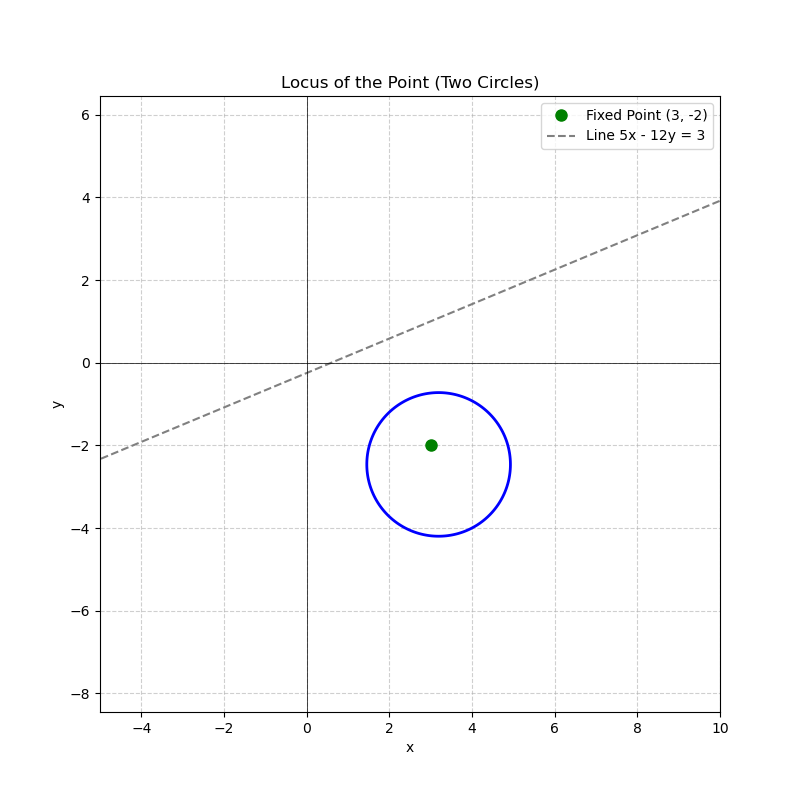
\includegraphics[width=0.7
    \linewidth]{Beamer/figs/circle.png}
    \caption{}
    \label{fig:placeholder}
\end{figure}

\end{frame}





\end{document}



